%!TEX root = origin.TEX
\frame{\titlepage}

\AtBeginSection[]{
\begin{frame}
\frametitle{
\begin{center}
{Modelo De Reconocimiento Automático De Señales De Tránsito Vehicular Mediante Aprendizaje Profundo De Redes Neuronales Convolucionales}
\end{center}
}
\tableofcontents[currentsection]
\end{frame}
}

\frame{
\begin{abstract}
\justifying
\begin{center}
Esta investigación pretende contribuir en la industria automotriz, especificamente en los campos de construcción de vehículos autónomos y de los sistemas avanzados de asistencia al conductor, iniciando con la adquisición de imágenes, luego para el pre-procesamiento, se implementará algoritmos de realce de contraste, reducción de ruido, rotación y proyecciones de escalamiento con la finalidad de aumentar el conjunto de datos y poder ejecutar el aprendizaje profundo a través de arquitecturas de redes neuronales convolucionales. Se realizaron diferentes diseños de arquitecturas convolucionales y se escogió el que obtuvo los mejores indicadores/resultados.
\vskip 0.8cm
\hspace*{0.0cm}{\bf Palabras claves:} aprendizaje profundo, redes neuronales convolucionales, procesamiento de imágenes.
\end{center}
\end{abstract}
}

%-------------------------------------------------------------------------------------------------
%-------------------------------------------------------------------------------------------------
\section{Introducción}
	\frame{
	\begin{block}
	{\Large{Introducción}}
	\end{block}
	\vskip 0.5cm
	\begin{itemize}
		
		\item<1->Al conducir en carreteras congestionadas, a veces es difícil mantener los ojos en todas partes a la vez, comprobando el camino por delante, el tráfico venidero, lo que está detrás de usted, tratar de mantener la velocidad permitida; es por ello, que existen mecanismos destinados a reglamentar el tránsito, advertir o informar a los usuarios mediante palabras, sonidos o símbolos determinados.

		\item<2->La policía de tránsito o las {\bf señalizaciones vehiculares} que según sea el caso, en todos los países regulan el tránsito e informan al usuario sobre direcciones, rutas, destinos, así como dificultades existentes en las carreteras y previenen cualquier peligro que podría presentarse en la circulación vehicular.

	\end{itemize}
	}

	\frame{
	\begin{block}
	{\Large{Introducción}}
	\end{block}
	\vskip 0.5cm
	\begin{itemize}
		
		\item<1-> La inseguridad vial es un problema de interés mundial, según el último informe de la OMS (Organización Mundial de la salud) anualmente cerca de 1,3 millones de personas mueren alredor del mundo y entre 20 y 50 millones padecen traumatismos no mortales,\citep{OMS}. Son distintas las causas que conllevan a este problema, de las cuales las principales pueden ser la falta de concientización y educación vial.
	\end{itemize}
	}

	\frame{
	\begin{block}
	{\Large{Introducción}}
	\end{block}
	\vskip 0.5cm
	\begin{itemize}
		
		\item<1-> El Perú y la capital Lima se encuentran respectivamente en la lista de peores países y ciudades para conducir en America Latina, según el Índice Global de Satisfacción del Conductor \citep{CNN}, lo cual se ve reflejado en que los últimos años se ha incrementado el índice de mortandad originados por los accidentes de tránsito siendo las principales causas de los mismos el exceso de velocidad, estado de ebriedad del conductor y sobretodo el desacato a las señales de tránsito, todas ellas de responsabilidad directa del conductor del vehículo motorizado,\citep{SUTRAN}. 
		 
		\item<2-> Es por ello que trabajar en obtener vehículos más seguros es un factor fundamental para prevenir de alguna forma los accidentes de tránsito o reducir la probabilidad de que estos sean producidos, \citep{OMS}.
		
	\end{itemize}
	}

%-------------------------------------------------------------------------------------------------
%-------------------------------------------------------------------------------------------------

\section{Motivación}
	\frame{
	\begin{block}
	{\Large{Motivación}}
	\end{block}
	\vskip 0.2cm
	\begin{itemize}
		\item<1-> Para contribuir con lo antes mencionado, se han venido planteando formas que permitan la asistencia en el reconocimiento de señales de tránsito, la cual es un problema de clasificación multicategórica que comúnmente presenta desigualdades en las frecuencias de aparición de las categorías. Además, las señales de tránsito muestran una amplia gama de variaciones entre las clases en términos de color, forma, subconjuntos de clases que son muy similares entre sí y la presencia de símbolos, leyendas o texto. A esto es sumado, las grandes variaciones en las apariencias visuales debido a cambios de iluminación, oclusiones parciales, rotaciones, condiciones meteorológicas, escalamiento, etc. 

		\item<2-> Todo esto representa un reto para el reconocedor/clasificador de señales de tránsito vehicular y es por ello que se han venido realizando diversas investigaciones, donde esta forma parte de una de ellas.
	\end{itemize}
	}
%-------------------------------------------------------------------------------------------------
%-------------------------------------------------------------------------------------------------
\section{Formulación del problema}
	\frame{
	\begin{block}
	{\Large{Formulación del problema}}
	\end{block}
	\vskip 0.3cm
	 En este trabajo, se propone discutir el modelo de redes neuronales convolucionales basado en el problema del reconocimiento de imágenes para responder a la siguiente pregunta:
	 \vskip 0.3cm
	 \begin{center} 
	     ¿Cómo se puede reconocer de manera automática señales de tránsito vehicular?
	 \end{center}
	}
%-------------------------------------------------------------------------------------------------
%-------------------------------------------------------------------------------------------------

\section{Importancia de la investigación} 
	\frame{
	\vskip -1cm
	\begin{block}
	{\Large{Importancia de la investigación - Justificación Académica}}
	\end{block}
	\vskip 0.3cm
	\begin{itemize}
	\item<1->  La importancia de esta investigación en el punto de vista de ciencias de la computación se justifica en poner en práctica los conocimientos adquiridos en la formación académica, siendo los más resaltables el tema de procesamiento de imágenes, cálculo matemático e inteligencia artificial con la finalidad de obtener un modelo robusto de redes neuronales convolucionales basadas en el aprendizaje profundo (deep learning) que permita analizar el contenido de imágenes para el reconocer de señales de tránsito vehicular.   
	\vskip 0.15cm
	\item<2-> En este sentido, esta investigación pretende la elaboración de un modelo basado en el aprendizaje profundo de redes convolucionales que permita el reconocimiento de señales de tránsito vehicular. La siguiente figura muestra un diagrama de bloques con la secuencia de actividades que demanda el reconocimiento.
	\end{itemize}
	}


	\frame{
	\vskip -1cm
	\begin{block}
	{\Large{Importancia de la investigación - Justificación Académica}}
	\end{block}
	\vskip 0.3cm
		\begin{figure}[H]
		\begin{center}
		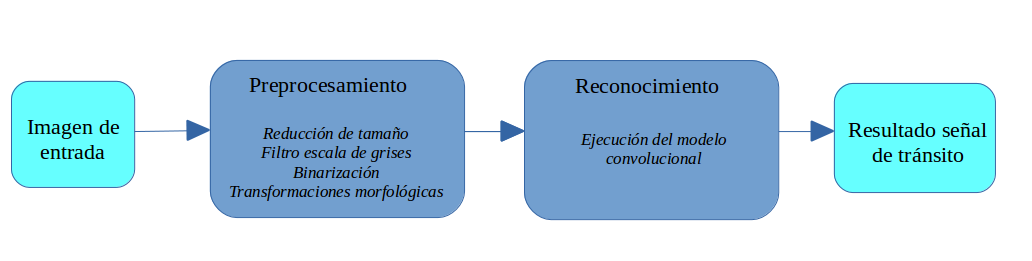
\includegraphics[width=0.8\textwidth]{images/intro/bloque}
		\end{center}
		\begin{center}
		\caption{\small{Diagrama de bloques del modelo prentedido}}
		{\small{Fuente propia}}
		\end{center}
		\vspace{-1.5em}
		\end{figure}
	}

	\frame{
	\vskip -1cm
	\begin{block}
	{\Large{Importancia de la investigación - Justificación Social}}
	\end{block}
	\vskip 0.3cm
	\begin{itemize}
	\item<1->  Teniendo conocimiento de lo descrito en la realidad problemática, la visibilidad y conocimiento de señales de tráfico es crucial para la seguridad de los conductores y es por ello que la introducción de un modelo de reconocimiento de señales de tránsito que funcione en diferentes contextos puede formar parte de la solución a que constantes infracciones y muertes se puedan evitar y en consecuencia reducir estos indices progresivamente.  
	\vskip 0.2cm
	
	\item<2-> A continuación algunos ejemplos:
	\vskip 0.2cm
	\begin{enumerate}	
		\item[--]<3-> Dar una notificación al no darse cuenta de un cambio en el límite de velocidad
		 \vskip 0.2cm
		\item[--]<4-> El aviso de que se está comentiendo una infracción al girar o estacionarse donde no se debe 
	\end{enumerate} 
	\end{itemize}
	}

	\frame{
	\vskip -1cm
	\begin{block}
	{\Large{Importancia de la investigación - Justificación Social}}
	\end{block}
	\vskip 0.3cm
	\begin{itemize}
	\item<1->
		\begin{enumerate}
		\item[--]<2-> La advertencia de un peligro potencial por delante.
		\vskip 0.2cm
		\item[--]<3-> Una aplicación móvil que dé la posibilidad de reconocer automáticamente aquella señal de tránsito que usuarios puedan desconocer serviría como aporte en la educación vial. 
		\vskip 0.2cm
		\item[--]<4-> Podría ser un componente útil en cámaras de video vigilancia convirtiendolas en más inteligentes con la capacidad de monitorear que las señales de tránsito sean respetadas.
		\end{enumerate} 
	\vskip 0.2cm
	
		\item<5-> En este sentido, esta investigación pretende la elaboración de un modelo basado en el aprendizaje profundo de redes convolucionales que permita el reconocimiento de señales de tránsito vehicular. La siguiente figura muestra un diagrama de bloques con la secuencia de actividades que demanda el reconocimiento.
	\end{itemize}
	}
%-------------------------------------------------------------------------------------------------
%-------------------------------------------------------------------------------------------------



\section{Contribución de la investigación}
\frame{
\begin{block}
{\Large{Contribución de la investigación}}
\end{block}
\vskip 0.5cm
\begin{itemize}
\item<1->Todos los hechos descritos hacen que el reconocimiento de las señales de tránsito sea un reto desafiante y esencial en muchos aspectos, no solo para contribuir en los esfuerzos de la industria automotriz en el campo de la asistencia al conductor, sino también para organismos internacionales y gubernamentales quienes se dan cuenta de la problemática que representa la inseguridad vial y buscan constantemente introducir nuevos mecanismos y tecnologías que faciliten y mejoren la conducción vehicular para el beneficio propio del conductor y en general para la seguridad vial de la sociedad.
\end{itemize}
}
%-------------------------------------------------------------------------------------------------
%-------------------------------------------------------------------------------------------------

